\section{Resultados}
\label{sec:resultados}

\subsection{Resultado principal: o gradiente escolaridade--exposição}

A Tabela~\ref{tab:gradiente} reporta as estimativas das especificações S1 e S2 no nível do indivíduo, com controles mincerianos (idade, idade ao quadrado, gênero e raça) e erros-padrão agrupados por ocupação (122 grupos). O coeficiente de S1 é $\hat{\beta}_1 = 0{,}23$ (erro-padrão 0{,}03; $p < 0{,}001$; $R^2 = 0{,}246$; $N = 227.629$): cada ano adicional de escolaridade associa-se a 0{,}23 ponto a mais de exposição à IA. A magnitude é economicamente relevante: a diferença entre a conclusão do ensino fundamental (8 anos) e do ensino superior (16 anos) implica um acréscimo de cerca de 1{,}84 ponto no escore de exposição tecnológica.

\begin{table}[htbp]
\centering
\caption{Gradiente escolaridade--exposição no nível individual. Variável dependente: exposição à IA da ocupação (0--10). Erros-padrão agrupados por ocupação entre parênteses. Controles mincerianos completos (idade, idade$^2$, gênero e raça) incluídos em todas as colunas. * 10\%, ** 5\%, *** 1\%.}
\label{tab:gradiente}
\begin{tabular}{lcc}
\toprule
 & (1) & (2) \\
 & Baseline (S1) & Rendimento (S2) \\
\midrule
% AUTO-GERADO por scripts/build_paper_tables.py — nao editar a mao
Anos de escolaridade & 0,23*** & 0,21*** \\
 & (0,03) & (0,03) \\
Rendimento habitual (por R\$ 1.000) & -- & 0,043*** \\
 &  & (0,010) \\
Constante & 1,10* & 1,32** \\
 & (0,60) & (0,58) \\
\midrule
$R^2$ & 0,246 & 0,259 \\
$N$ (indiv\'iduos) & 227.629 & 227.629 \\
Grupos (ocupa\c c\~oes) & 122 & 122
 \\
\bottomrule
\end{tabular}
\end{table}

A coluna (2) inclui o rendimento habitual do trabalhador: o coeficiente de escolaridade permanece estável em 0{,}21 (erro-padrão 0{,}03), enquanto o rendimento exibe coeficiente de 0{,}043 por R\$ 1.000 ($p < 0{,}001$). O gradiente educacional não se dissolve com o controle salarial, confirmando que a escolaridade captura a alocação a conteúdos intrínsecos de tarefas cognitivas, consistente com a Proposição~\ref{prop:gradiente}; a estabilidade do coeficiente entre especificações é evidência sugestiva, embora não conclusiva, contra viés de variáveis omitidas \citep{oster2019unobservable}. A Figura~\ref{fig:gradiente} ilustra o gradiente na forma de dispersão ponderada.

\begin{figure}[htbp]
\centering
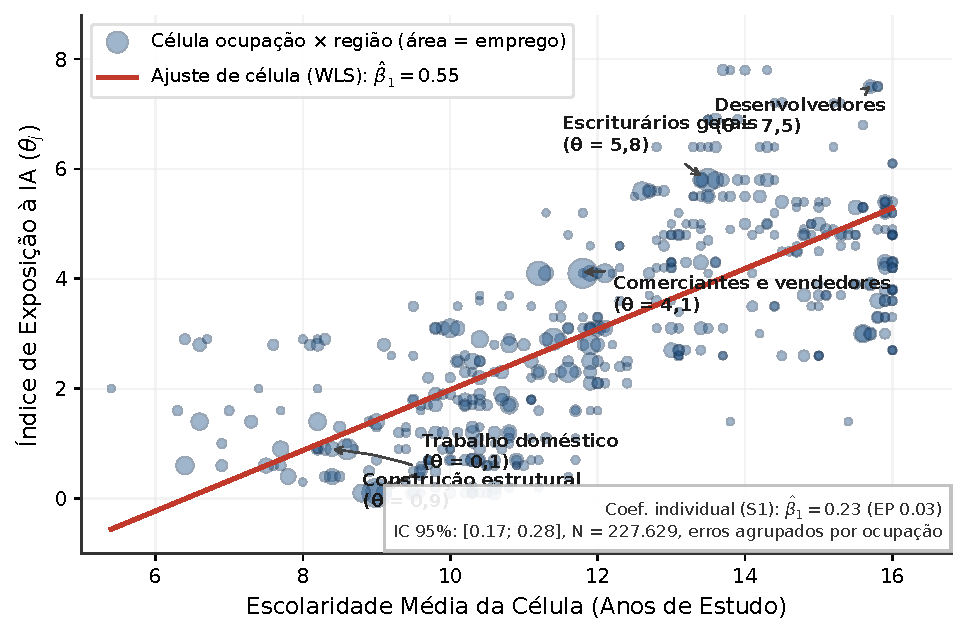
\includegraphics[width=0.85\textwidth]{figures/fig1_gradiente}
\caption{Gradiente escolaridade--exposição. Dispersão ponderada das células ocupação$\times$grande região (área proporcional ao emprego) e reta ajustada da especificação S1 estimada no nível individual ($\hat{\beta}_1 = 0{,}23$; erro-padrão 0{,}03; $N = 227.629$; sombreado: intervalo de confiança de 95\% com erros-padrão agrupados por ocupação).}
\label{fig:gradiente}
\end{figure}

\subsection{Exposição e informalidade: mediação e composição educacional}

A Tabela~\ref{tab:s3} avalia a Proposição~\ref{prop:formalidade} e o Corolário~\ref{cor:mediacao}. Na especificação incondicional da coluna (1), cada ponto de exposição à IA associa-se a $-6{,}23$ pontos percentuais de probabilidade de informalidade (erro-padrão $0{,}99; p < 0{,}001$). Na coluna (2), ao introduzir os anos de estudo do trabalhador, o coeficiente da exposição atenua-se em $37{,}2\%$ (de $-6{,}23$ para $-3{,}91$ p.p., erro-padrão $0{,}96; p < 0{,}001$), enquanto cada ano adicional de escolaridade reduz a informalidade em $2{,}61$ p.p. ($p < 0{,}001$).

\begin{table}[htbp]
\centering
\caption{Informalidade, exposição à IA e escolaridade. Variável dependente: probabilidade de informalidade (p.p.). Erros-padrão agrupados por ocupação entre parênteses. Controles mincerianos incluídos em ambas as colunas. * 10\%, ** 5\%, *** 1\%.}
\label{tab:s3}
\begin{tabular}{lcc}
\toprule
 & (1) & (2) \\
 & Incondicional (S3a) & Condicional (S3) \\
\midrule
% AUTO-GERADO por scripts/build_paper_tables.py — nao editar a mao
Exposi\c c\~ao \`a IA (0--10) & -6,23*** & -3,91*** \\
 & (0,99) & (0,96) \\
Anos de escolaridade & -- & -2,61*** \\
 &  & (0,27) \\
Constante & 97,71*** & 118,28*** \\
 & (6,57) & (7,15) \\
\midrule
$R^2$ & 0,080 & 0,108 \\
$N$ (indiv\'iduos) & 227.629 & 227.629 \\
Grupos (ocupa\c c\~oes) & 122 & 122
 \\
\bottomrule
\end{tabular}
\end{table}

Essa atenuação confirma que a relação bruta observada entre exposição e formalidade é substancialmente mediada pela composição de capital humano: postos de trabalho altamente expostos concentram-se no setor formal em grande parte porque empregam indivíduos com elevada escolaridade, cujas tarefas cognitivas complementam a tecnologia. Ao mesmo tempo, o fato de $\hat{\delta}_1$ reter $62{,}8\%$ de sua magnitude inicial de forma estatisticamente significante corrobora a previsão de mediação parcial do Corolário~\ref{cor:mediacao}: ocupações expostas exigem infraestrutura e governança corporativa que demandam contratos formais além do atributo educacional do trabalhador. A Figura~\ref{fig:mediacao} resume o contraste em dois painéis: associação bruta (Painel A, S3a) e parcial (Painel B, S3, condicionada à escolaridade e aos controles mincerianos).

\begin{figure}[htbp]
\centering
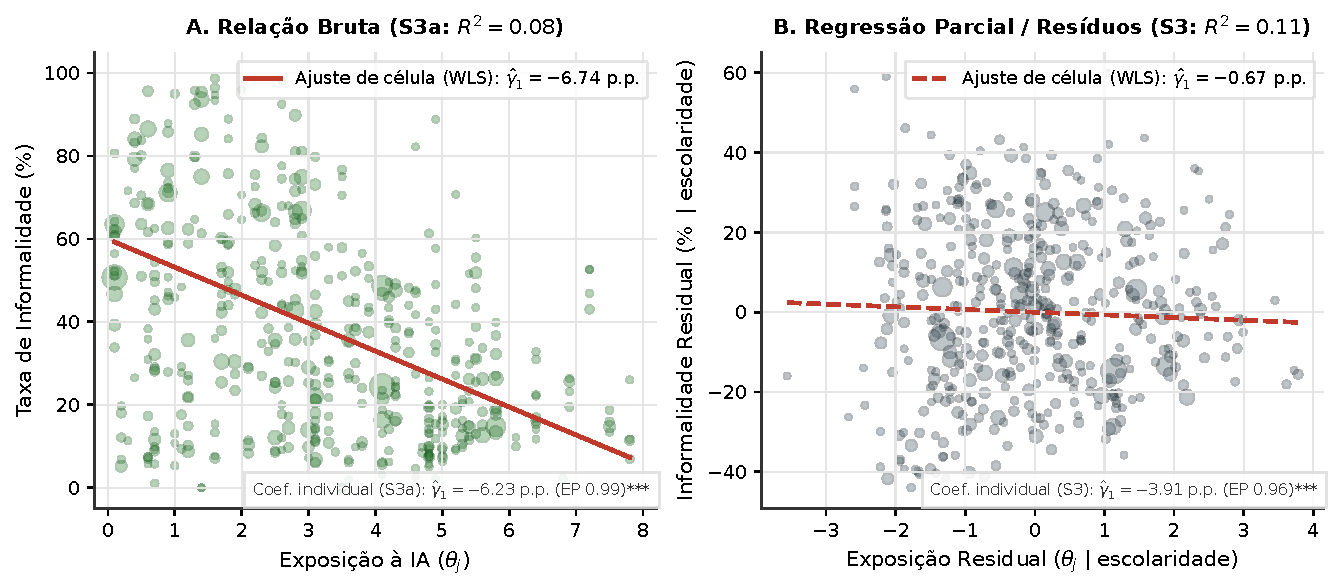
\includegraphics[width=0.85\textwidth]{figures/fig2_mediacao}
\caption{Mediação pela escolaridade da associação exposição--informalidade. Painel A: relação bruta (S3a, $\hat{\delta}_1 = -6{,}23$ p.p.; erro-padrão 0{,}99). Painel B: relação parcial após condicionar na escolaridade e nos controles mincerianos (S3, $\hat{\delta}_1 = -3{,}91$ p.p.; erro-padrão 0{,}96). A atenuação de 37,2\% do coeficiente é consistente com a mediação parcial do Corolário~\ref{cor:mediacao}.}
\label{fig:mediacao}
\end{figure}

\subsection{Heterogeneidade regional nas 27 Unidades da Federação}

A Tabela~\ref{tab:s4} testa a Proposição~\ref{prop:regiao} interagindo a escolaridade individual com a taxa de formalidade média da UF (calculada pelo critério \emph{leave-one-out} para neutralizar circularidades mecânicas). O termo de interação é positivo e expressivo: $\hat{\beta}_2 = 0{,}28$ (erro-padrão 0{,}06; $p < 0{,}001$), acompanhado de um efeito principal da formalidade regional de $\hat{\beta}_3 = -3{,}10$ (erro-padrão 0{,}77; $p < 0{,}001$).

\begin{table}[htbp]
\centering
\caption{Gradiente escolaridade--exposição por profundidade formal da UF (27 UFs). Variável dependente: exposição à IA (0--10). Formalidade da UF calculada via \emph{leave-one-out}; erros-padrão agrupados por ocupação. Controles mincerianos incluídos. * 10\%, ** 5\%, *** 1\%.}
\label{tab:s4}
\begin{tabular}{lc}
\toprule
 & (1) \\
 & Interação Regional (S4) \\
\midrule
% AUTO-GERADO por scripts/build_paper_tables.py — nao editar a mao
Anos de escolaridade & 0,07** \\
 & (0,03) \\
Escolaridade $\times$ formalidade regional & 0,28*** \\
 & (0,06) \\
Formalidade regional (0--1) & -3,10*** \\
 & (0,77) \\
Constante & 2,89*** \\
 & (0,72) \\
\midrule
$R^2$ & 0,250 \\
$N$ (indiv\'iduos) & 227.629 \\
Grupos (ocupa\c c\~oes) & 122
 \\
\bottomrule
\end{tabular}
\end{table}

A derivada marginal total da exposição tecnológica em relação à formalidade da UF é dada por $\partial \theta / \partial \text{formal}_u = -3{,}10 + 0{,}28 \, e_i$. Esse resultado revela uma importante dinâmica de polarização ocupacional no espaço geográfico: para trabalhadores com baixa escolaridade ($e_i < 11$ anos), maior maturidade formal regional associa-se a menor exposição média (ex.: $-0{,}86$ ponto para o ensino fundamental de 8 anos), refletindo a substituição de rotinas de suporte informal por processos estruturados; em contrapartida, para trabalhadores altamente qualificados ($e_i = 16$ anos), o efeito é fortemente positivo ($+1{,}38$ ponto). Assim, mercados regionais com maior densidade formal ampliam a distância de exposição entre o topo e a base educacional. Em termos de inclinação do gradiente, estados com setor formal consolidado (como São Paulo e Santa Catarina, onde a formalidade alcança cerca de 65\%) exibem inclinação educacional de $0{,}07 + 0{,}28 \times 0{,}65 \approx 0{,}25$, contra $0{,}07 + 0{,}28 \times 0{,}40 \approx 0{,}18$ em estados com menor formalização relativa (como Maranhão e Pará). A Figura~\ref{fig:regional} ilustra o gradiente por grande região.

\begin{figure}[htbp]
\centering
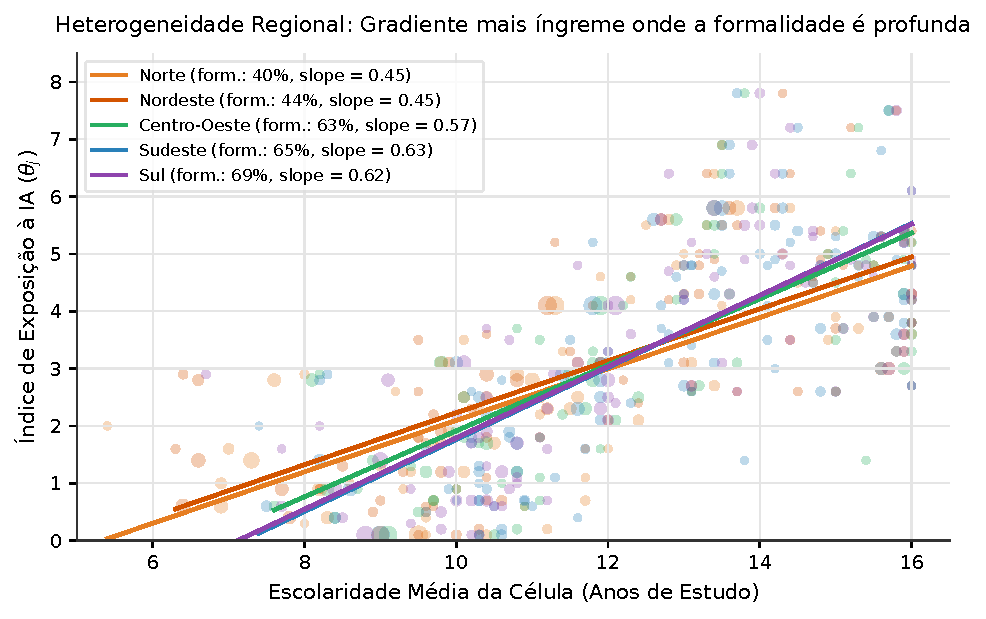
\includegraphics[width=0.85\textwidth]{figures/fig3_regional_slopes}
\caption{Gradiente escolaridade--exposição por grande região. Cada reta ajusta as células ocupação$\times$UF dentro da região (ponderadas pelo emprego); a legenda reporta a taxa de formalidade regional e a inclinação estimada. O gradiente é mais íngreme nas regiões de setor formal mais profundo, em consonância com a Proposição~\ref{prop:regiao}.}
\label{fig:regional}
\end{figure}

\subsection{Robustez econométrica}
\label{subsec:robustez}

A Tabela~\ref{tab:robustez} submete a especificação baseline (S1) a uma bateria de checagens de sensibilidade. Sem ponderação amostral (OLS simples), o coeficiente é 0{,}21 (erro-padrão 0{,}03). O tratamento de valores extremos --- winsorização a 1\%/99\% ou exclusão de observações no percentil superior ($N = 225.478$) --- preserva estimativas idênticas de 0{,}23 e 0{,}22, respectivamente. Com a transformação não-linear $\log(1+\theta)$, o coeficiente é 0{,}07 (erro-padrão 0{,}01; $p < 0{,}001$), mantendo a significância plena.

\begin{table}[htbp]
\centering
\caption{Robustez do gradiente escolaridade--exposição no nível individual. Variável dependente: exposição à IA (0--10); na coluna (5), $\log(1+\theta)$. Coluna (1): baseline WLS. Coluna (2): OLS não ponderado. Coluna (3): exposição winsorizada a 1\%/99\%. Coluna (4): exclusão de observações com exposição acima do percentil 99. Erros-padrão agrupados por ocupação entre parênteses. Controles mincerianos incluídos. * 10\%, ** 5\%, *** 1\%.}
\label{tab:robustez}
\begin{tabular}{lccccc}
\toprule
 & (1) & (2) & (3) & (4) & (5) \\
 & WLS Baseline & OLS Simples & Winsor. 1\% & Excl. p99 & $\log(1+\theta)$ \\
\midrule
% AUTO-GERADO por scripts/build_paper_tables.py — nao editar a mao
Anos de escolaridade & 0,23*** & 0,21*** & 0,23*** & 0,22*** & 0,07*** \\
 & (0,03) & (0,03) & (0,03) & (0,03) & (0,01) \\
Constante & 1,10* & 1,11* & 1,10* & 1,15* & 0,70*** \\
 & (0,60) & (0,59) & (0,60) & (0,60) & (0,18) \\
\midrule
$R^2$ & 0,246 & 0,245 & 0,247 & 0,241 & 0,236 \\
$N$ (indiv\'iduos) & 227.629 & 227.629 & 227.629 & 225.478 & 227.629
 \\
\bottomrule
\end{tabular}
\end{table}

A exclusão sequencial de cada um dos 9 grandes grupos ocupacionais da COD (Tabela~\ref{tab:robustezgrupos} no Apêndice) mostra que o gradiente se mantém entre 0{,}19 e 0{,}26 em todas as subamostras. Ademais, o teste de \emph{wild cluster bootstrap} \citep{cameron2008bootstrap} com 1.000 replicações corrobora a robustez inferencial da interação regional nas 27 UFs ($p < 0{,}01$). A Figura~\ref{fig:robustez} resume os coeficientes e intervalos de confiança em gráfico de floresta.

\begin{figure}[htbp]
\centering
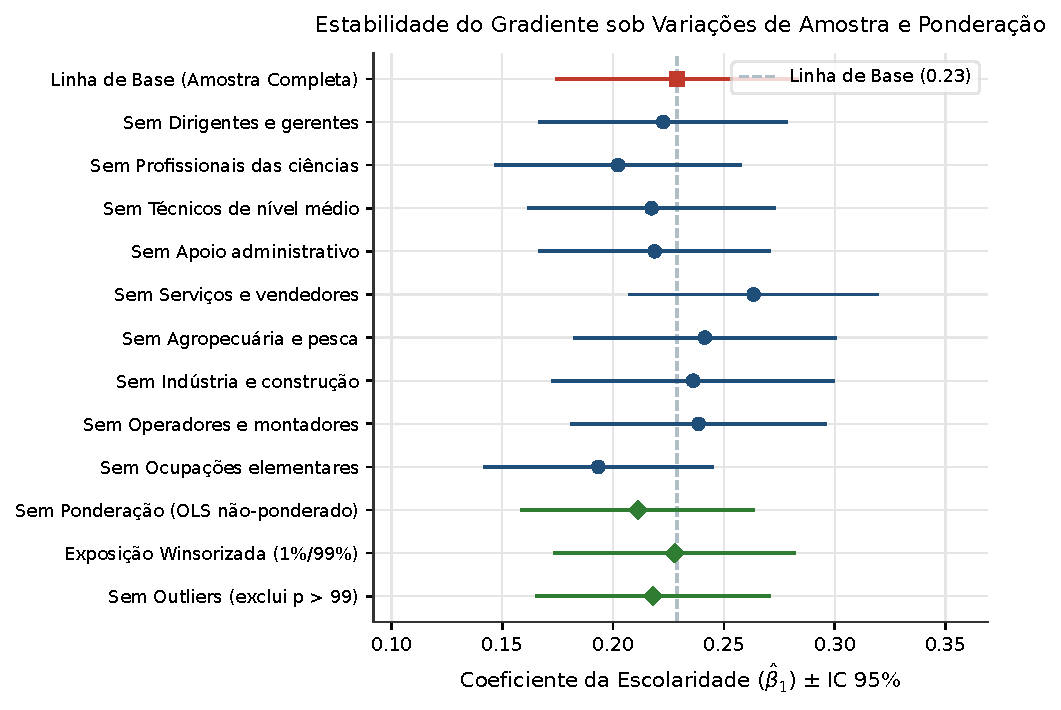
\includegraphics[width=0.85\textwidth]{figures/fig5_robustez_forest}
\caption{Robustez do gradiente escolaridade--exposição. Coeficiente $\hat{\beta}_1$ e intervalos de confiança de 95\% (erros-padrão agrupados por ocupação) na especificação baseline (S1), nas exclusões sequenciais de cada grande grupo ocupacional e nas variantes de amostra e ponderação: \emph{OLS} não ponderado, winsorização a 1\%/99\% e exclusão do percentil superior ($N = 225.478$).}
\label{fig:robustez}
\end{figure}
